% ---- Double-column (full text width) ----
\begin{figure*}[t]
  \centering
  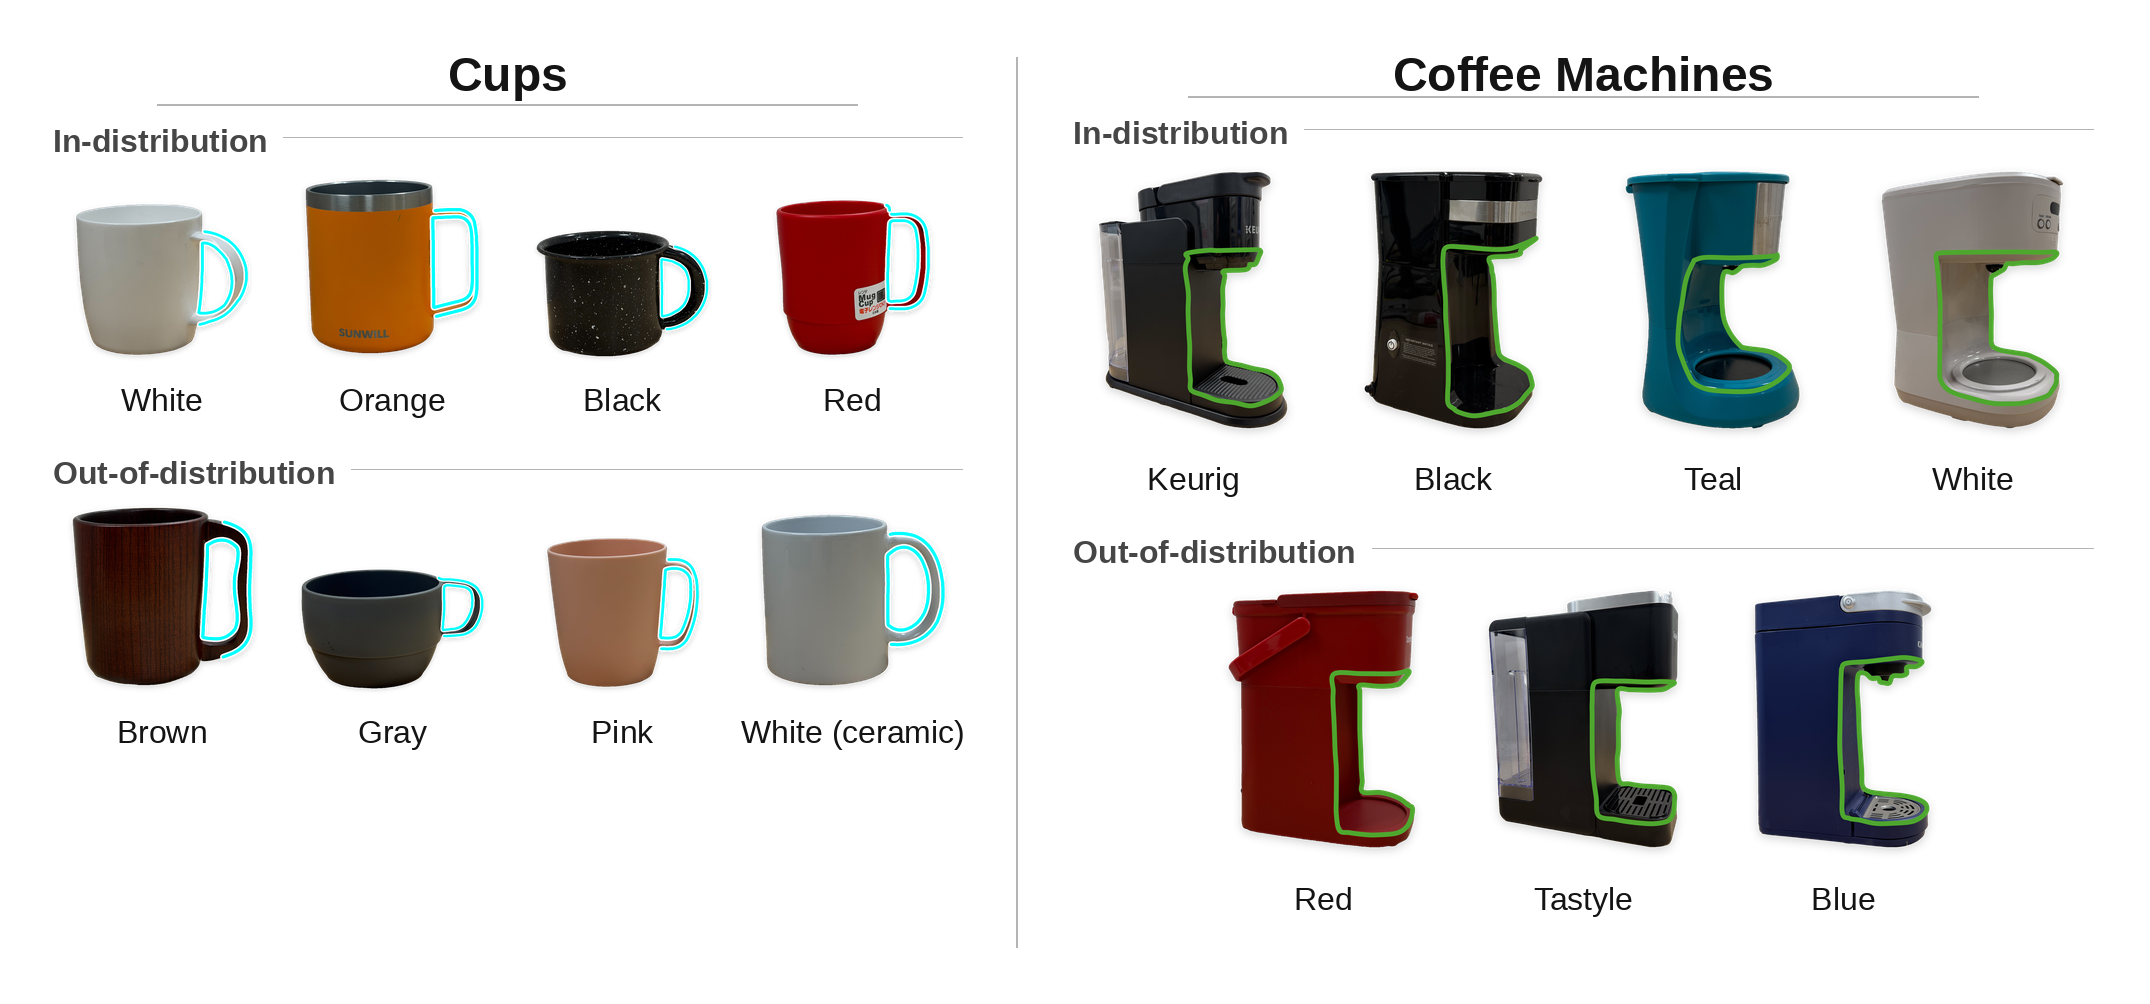
\includegraphics[width=\textwidth]{figure_collection_2col.png}
  \caption{\textbf{Object collection for the mug pick-and-place task.}
  Each policy and robot arm is evaluated on grasping a mug and placing it on a
  coffee machine. We test across a set of \emph{cups} (left) and \emph{coffee
  machines} (right), each split into in-distribution instances seen during
  training and out-of-distribution instances held out for evaluation. The cups
  span a wide range of \textbf{handle geometries} (traced in cyan)---rounded
  loop handles, square and D-shaped handles, and compact ear handles---together
  with differences in size, body taper and diameter, wall thickness, material
  (plastic, ceramic, enamel, wood, and vacuum-insulated steel), and color. The
  coffee machines differ in overall height, body and base geometry, the shape of
  the cup-placement platform, and the vertical clearance between the platform and
  the dispenser head---all of which constrain where and how a cup can be placed.
  For each machine we highlight in green the \textbf{cup-clearance pocket}: the
  contour-bounded region a placed mug must fit into, spanning the platform, the
  inner wall, and the underside of the dispenser.
  In-distribution cups: white, orange, black, red; out-of-distribution: brown,
  gray, pink, and white ceramic. In-distribution machines: Keurig, black, teal,
  and white; out-of-distribution: red, Tastyle, and blue.}
  \label{fig:object_collection}
\end{figure*}

% ---- Single-column variant ----
% \begin{figure}[t]
%   \centering
%   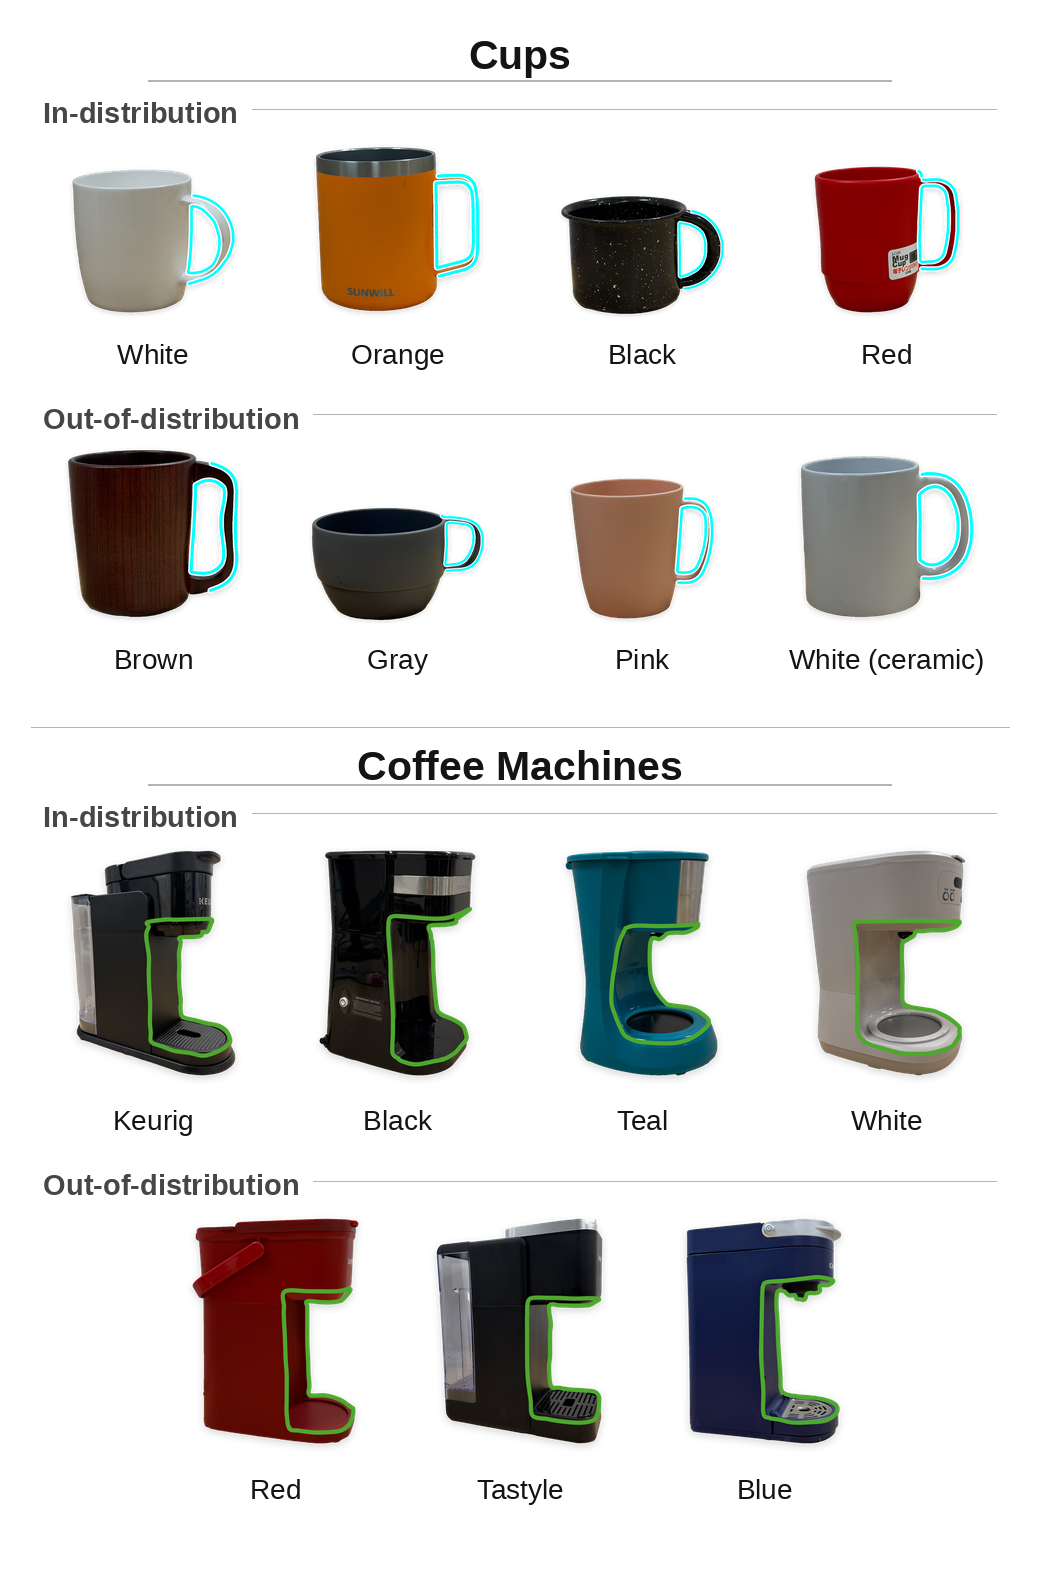
\includegraphics[width=\columnwidth]{figure_collection_1col.png}
%   \caption{... same caption as above ...}
%   \label{fig:object_collection}
% \end{figure}
